\documentclass{article}
\iffalse
This file is protected by Copyright. Please refer to the COPYRIGHT file
distributed with this source distribution.

This file is part of OpenCPI <http://www.opencpi.org>

OpenCPI is free software: you can redistribute it and/or modify it under the
terms of the GNU Lesser General Public License as published by the Free Software
Foundation, either version 3 of the License, or (at your option) any later
version.

OpenCPI is distributed in the hope that it will be useful, but WITHOUT ANY
WARRANTY; without even the implied warranty of MERCHANTABILITY or FITNESS FOR A
PARTICULAR PURPOSE. See the GNU Lesser General Public License for more details.

You should have received a copy of the GNU Lesser General Public License along
with this program. If not, see <http://www.gnu.org/licenses/>.
\fi

\author{} % Force author to be blank
%----------------------------------------------------------------------------------------
% Paper size, orientation and margins
%----------------------------------------------------------------------------------------
\usepackage{geometry}
\geometry{
	letterpaper,			% paper type
	portrait,				% text direction
	left=.75in,				% left margin
	top=.75in,				% top margin
	right=.75in,			% right margin
	bottom=.75in			% bottom margin
 }
%----------------------------------------------------------------------------------------
% Header/Footer
%----------------------------------------------------------------------------------------
\usepackage{fancyhdr} \pagestyle{fancy} % required for fancy headers
\renewcommand{\headrulewidth}{0.5pt}
\renewcommand{\footrulewidth}{0.5pt}
\rhead{\small{ANGRYVIPER Team}}
%----------------------------------------------------------------------------------------
% Appendix packages
%----------------------------------------------------------------------------------------
\usepackage[toc,page]{appendix}
%----------------------------------------------------------------------------------------
% Defined Commands & Renamed Commands
%----------------------------------------------------------------------------------------
\renewcommand{\contentsname}{Table of Contents}
\renewcommand{\listfigurename}{List of Figures}
\renewcommand{\listtablename}{List of Tables}
\newcommand{\todo}[1]{\textcolor{red}{TODO: #1}\PackageWarning{TODO:}{#1}} % To do notes
\newcommand{\code}[1]{\texttt{#1}} % For inline code snippet or command line
%----------------------------------------------------------------------------------------
% Various pacakges
%----------------------------------------------------------------------------------------
\usepackage{hyperref} % for linking urls and lists
\usepackage{graphicx} % for including pictures by file
\usepackage{listings} % for coding language styles
\usepackage{rotating} % for sideways table
\usepackage{pifont}   % for sideways table
\usepackage{pdflscape} % for landscape view
%----------------------------------------------------------------------------------------
% Table packages
%----------------------------------------------------------------------------------------
\usepackage{tabularx} % c=center,l=left,r=right,X=fill
\usepackage{float}
\floatstyle{plaintop}
\usepackage[tableposition=top]{caption}
\newcolumntype{P}[1]{>{\centering\arraybackslash}p{#1}}
\newcolumntype{M}[1]{>{\centering\arraybackslash}m{#1}}
%----------------------------------------------------------------------------------------
% Block Diagram / FSM Drawings
%----------------------------------------------------------------------------------------
\usepackage{tikz}
\usetikzlibrary{shapes,arrows,fit,positioning}
\usetikzlibrary{automata} % used for the fsm
%----------------------------------------------------------------------------------------
% Colors Used
%----------------------------------------------------------------------------------------
\usepackage{colortbl}
\definecolor{blue}{rgb}{.7,.8,.9}
\definecolor{ceruleanblue}{rgb}{0.16, 0.32, 0.75}
\definecolor{drkgreen}{rgb}{0,0.6,0}
\definecolor{deepmagenta}{rgb}{0.8, 0.0, 0.8}
\definecolor{cyan}{rgb}{0.0,0.6,0.6}
\definecolor{maroon}{rgb}{0.5,0,0}
%----------------------------------------------------------------------------------------
% Update the docTitle and docVersion per document
%----------------------------------------------------------------------------------------
\def\docTitle{Component Data Sheet}
\def\docVersion{1.3}
%----------------------------------------------------------------------------------------
\date{Version \docVersion} % Force date to be blank and override date with version
\title{\docTitle}
\lhead{\small{\docTitle}}

\def\comp{matchstiq\_z1\_avr}
\edef\ecomp{matchstiq_z1_avr}
\def\Comp{MATCHSTIQ\_Z1\_AVR}
\graphicspath{ {figures/} }

\begin{document}

\section*{Summary - \Comp}
\begin{tabular}{|c|M{13.5cm}|}
	\hline
	\rowcolor{blue}
	                  &                                        			\\
	\hline
	Name              & \comp                                  			\\
	\hline
	Worker Type       & Device                                 			\\
	\hline
	Version           & v\docVersion \\
	\hline
	Release Date      & February 2018 \\
	\hline
	Component Library & ocpi.assets.platforms.matchstiq\_z1.devices		\\
	\hline
	Workers           & \comp.hdl                              			\\
	\hline
	Tested Platforms  & Matchstiq-Z1(PL)                       			\\
	\hline
\end{tabular}

\section*{Worker Implementation Details}
On the Matchstiq-Z1 platform, there is an AVR microcontroller which contains platform information and controls platform peripherals via registers accessible via I2C transactions. The \Comp{} device worker uses the raw property interface to expose the features and hardware registers of the AVR microcontroller to the ANGRYVIPER framework.

\section*{Block Diagrams}
\subsection*{Top level}
\begin{figure}[ht]
	\centerline{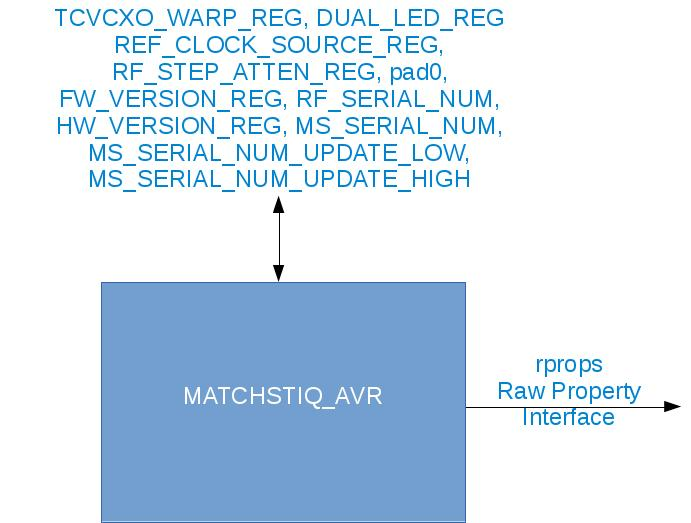
\includegraphics[scale=0.4]{matchstiq_z1_avr_top_level}}
	\label{fig:tb}
\end{figure}

\section*{Source Dependencies}
\subsection*{\comp.hdl}
\begin{itemize}
	\item ocpiassets/hdl/devices/\comp.hdl/\comp.vhd
\end{itemize}

\begin{landscape}
\section*{Component Spec Properties}
\begin{scriptsize}
		\begin{tabular}{|p{4cm}|p{1cm}|c|c|c|c|c|p{7cm}|}
			\hline
			\rowcolor{blue}
			Name               & Type   & SequenceLength & ArrayDimensions   & Accessibility       & Valid Range                                                                      & Default & Usage                                                                        \\
			\hline
			\verb+TCVCXO_WARP_REG+          & UShort  & - & -  & Writable & 648-3413 & 2048     & Register used for fine grained adjustments of the TCVCXO on Matchstiq-Z1 platform. \\
			\hline
			\verb+DUAL_LED_REG+             & UShort  & - & -  & Writable & 0-3      & 1        & Register used for controlling the LED on the front panel of the Matchstiq-Z1 platform. Bit 0 controls the green LED (0=off, 1=on) and bit 1 controls the red LED (0=off, 1=on). \\
			\hline
			\verb+REF_CLOCK_SOURCE_REG+     & UShort  & - & -  & Writable & -        & -        & \\
			\hline
			\verb+RF_STEP_ATTEN_REG+        & UShort  & - & -  & Writable & 0-63     & 0        & Register used to set the attenuation level of the programmable step attenuator in the RF receiver \\
			\hline
			\verb+pad0+                     & UShort  & - & 12 & Padding  & -        & -        & Unused address space \\
			\hline
			\verb+FW_VERSION_REG+           & UShort  & - & -  & Padding  & -        & -        & Firmware version register \\
			\hline
			\verb+RF_SERIAL_NUM+            & UShort  & - & -  & Padding  & -        & -        & RF serial number register \\
			\hline
			\verb+HW_VERSION_REG+           & UShort  & - & -  & Padding  & -        & -        & Hardware version register \\
			\hline
			\verb+MS_SERIAL_NUM+            & UShort  & - & -  & Volatile & -        & -        & Matchstiq serial number register \\
			\hline
			\verb+MS_SERIAL_NUM_UPDATE_LOW+ & UShort  & - & -  & Padding  & -        & -        & \\
			\hline
			\verb+MS_SERIAL_NUM_UPDATE_HIGH+& UShort  & - & -  & Padding  & -        & -        & \\
			\hline
		\end{tabular}
	\end{scriptsize}
	\section*{Worker Interfaces}
	\subsection*{\comp.hdl}
	\begin{scriptsize}
		\begin{tabular}{|M{2cm}|M{1.5cm}|c|c|M{12cm}|}
			\hline
			\rowcolor{blue}
			Type & Name & DataWidth & Advanced & Usage \\
			\hline
			RawProp
			& rprops
			& -
			& Master=true
			& \begin{flushleft}Raw properties connection for slave I2C device worker\end{flushleft}\\
			\hline
			ControlInterface
			& -
			& -
			& Timeout=131072
			& \begin{flushleft}Control clock cycles required to complete property  read/write. I2C transactions require additional clock cycles to complete than the default of 16 \end{flushleft}\\
			\hline
		\end{tabular}
	\end{scriptsize}
\end{landscape}

\section*{Control Timing and Signals}
The \Comp{} HDL device worker uses the clock from the Control Plane and standard Control Plane signals.

\section*{Performance and Resource Utilization}
\subsubsection*{\comp.hdl}
\input{../../\ecomp.hdl/utilization.inc}
\section*{Test and Verification}
There is no unit test for this device worker. The test and verification of this worker is covered in the Matchstiq I2C device worker. See the component datasheet of this worker for more details.
\end{document}
